In questo capitolo introduciamo notazioni formali e diamo una breve spiegazione del funzionamento delle reti neurali e degli strumenti utilizzati.

\section{Il Tempo}

Le RNN non sono limitate a sequenze indicizzate in maniera temporale.
Sono state usate con successo anche per sequenze di dati non temporali, come ad esempio i dati genetici.
In ogni caso, la computazione procede nel tempo e molte importanti applicazioni hanno un aspetto temporale esplicito o implicito.

Nonostante, in questa tesi, ci riferiremo al tempo i metodi descritti sono applicabili ad una famiglia pi\`u ampia di compiti.
Parlando di tempo ci riferiamo ad un campione $x^{(t)}$ in input e ad un valore atteso $y^{(t)}$ in output che sono generati in \emph{sequenze di fasi temporali} discrete indicate da $t$
La nostra sequenza pu\`o essere formata da un numero finito di campioni o da un numero infinito ma numerabile di campioni.
Se abbiamo a che fare con un numero finito di campioni allora possiamo indicare con $T$ il massimo indice temporale.
Quindi una sequenza di valori di input consecutivi pu\`o essere scritta come $(x^{(1)}, x^{(2)}, \dots, x^{(T)})$ mentre gli output come $(y^{(1)}, y^{(2)}, \dots, y^{(T)})$.
Questi valori possono essere dei campioni, presi ad intervalli regolari di tempo, di un processo reale continuo come ad esempio i fotogrammi che compongono un video.
Gli intervalli di tempo possono anche essere dei semplici valori ordinali senza una durata esatta.
\`E il caso, ad esempio, delle sequenze genetiche che hanno un ordine ma non un ordine temporale o ancora del linguaggio naturale dove le parole hanno un ordine logico ben preciso che, tuttavia, non corrisponde ad intervalli di temporali ben definiti.
Ad esempio nella frase ``\emph{Lisa suona il sassofono}'' abbiamo che $x^{(1)}$ = Lisa, $x^{(2)}$ = suona, ecc. Ciascuna parola corrisponde ad intervalli di tempo che non sono costanti, ``\emph{il}'' e ``\emph{sassofono}'' hanno bisogno di tempi diversi per essere pronunciati.

\section{Reti Neurali}
Le reti neurali sono modelli computazionali ispirati dalla biologia del sistema nervoso centrale.
Generalmente una rete neurale \`e formata da un insieme di \emph{neuroni artificiali}, comunemente chiamati \emph{nodi} o \emph{unit\`a}, collegati da un insieme di archi diretti che, intuitivamente, rappresentano le \emph{sinapsi} di una rete neurale biologica.
Associato ad ogni neurone $j$ vi \`e una funzione di attivazione $l_j$, chiamata anche funzione di collegamento (o funzione link).
In questa tesi user\`o la notazione ``$l_j$'' invece di ``$h_j$'' (notazione usata in altri documenti) per distinguere la funzione di attivazione $l_j$ dal valore dei nodi nascosti in una rete, che vengono comunemente indicati con \textbf{h} nella letteratura delle RNN.

Associato ad ogni arco dal nodo $j^{'}$ al nodo $j$ vi \`e un peso $w_{jj^{'}}$. Seguendo la convenzione adottata in molti altri documenti che trattano reti neurali, indicheremo i neuroni con $j$ e $j^{'}$ mentre, con $w_{jj^{'}}$, indicheremo il peso corrispondente all'arco diretto che parte dal nodo $j^{'}$ e arriva al nodo $j$.
\`E importante notare che in altri documenti e libri, come ad esempio su Wikipedia, gli indici dei pesi sono invertiti e che $w_{j^{'}j} \neq w_{jj^{'}}$ indica il peso sull'arco diretto dal nodo $j^{'}$ al nodo $j$.

Il valore $v_j$ di ciascun neurone $j$ \`e calcolato applicando la sua funzione di attivazione ad una somma pesata dei suoi valori di input (Fugura~\ref{fig:artificialNeuron}): %TODO pensare ad un titolo piu' appropiato
\begin{equation} % \begin{equantion*} per non numerare l'equazione
  v_j = l_j\left( \sum_{j^{'}} w_{jj^{'}} \cdot v_{j^{'}} \right)
\end{equation}

\begin{figure}[tp]
  \centering
  \begin{center}
    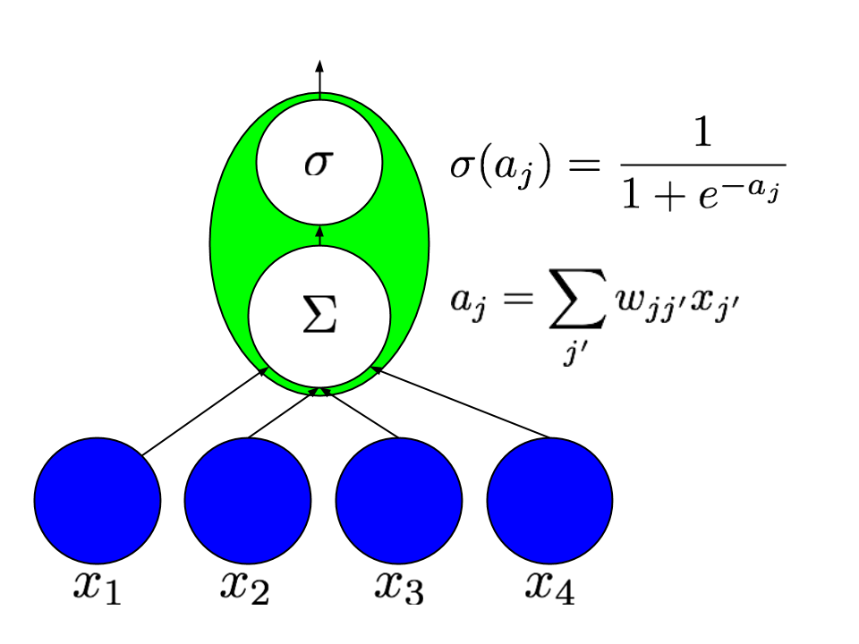
\includegraphics[width=0.7\textwidth]{./images/artificialNeuron.png}
  \end{center}
  \caption{Un neurone artificiale calcola una funzione non lineare della somma pesata dei suoi input}
  \label{fig:artificialNeuron}
\end{figure}
Per comodit\`a, ci riferiremo alla somma pesata all'interno delle parentesi come l'\emph{attivazione in arrivo} e la indicheremo con $a_j$. Rappresentiamo l'intero processo in figura disegnando i neuroni con dei cerchi mentre gli archi come delle frecce che li collegano.
Quando possibile, verr\`a utilizato un simbolo per indicare l'esatta funzione di attivazione utilizzata, ad esempio $\sigma$ per la funzione sigmoide.

Scelte abbastanza comuni per la funzione di attivazione includono la funzione sigmoide $\sigma(z) = 1/(1+e^{-z})$ e la funzione \emph{tanh} $\phi(z)=(e^z-e^{-z})/(e^z+e^{-z})$ che \`e diventata molto comune nelle reti neurali di tipo \emph{feedforward} ma \`e stata utilizzata anche in reti neurali ricorrenti~\cite{Sutskever:2011}.
Un'altra funzione di attivazione che \`e diventata lo stato dell'arte nella ricerca di deep learning \`e la funzione ReLU (\emph{rectified linear unit}) $l_j(z)=\operatorname{max}(0, z)$.
Questa funzione ha dimostrato di poter migliorare le prestazioni di molte reti neurali in una grande variet\`a di applicazioni, che spaziano dal riconoscimento vocale al riconoscimento di oggetti, ed \`e stata utilizzata anche in reti neurali ricorrenti~\cite{Bengio:2013}.

La funzione di attivazione da applicare sui nodi di output dipende dall'applicazione.
Per una classificazione a pi\`u classi, applichiamo al livello di output una funzione non lineare softmax.
La funzione softmax calcola l'output come:
\begin{equation}
  \hat{y_k} = \frac{e^{a_k}}{\sum_{k^{'}=1}^{K} e^{a_{k^{'}}}}
\end{equation}
dove $K$ \`e il numero totale di possibili output (classi). Il denominatore \`e una funzione di normalizzazione che consiste nella somma di funzioni esponenziali dei valori dati in output da tutti i nodi e serve per assicurarsi che l'output totale sommi ad 1.
Nel caso di regressioni invece viene comunemente utilizzata una funzione lineare come output.
Dato che nella maggioranza dei casi le reti neurali, specialmente quelle ricorrenti, vengono utilizzate per applicazioni che coinvolgono la classificazione, durante questa tesi, a meno che diversamente specificato, daremo per scontato l'uso della funzione softmax come output.

\section{Reti Neurali Feedforward}
Con un modello computazionale a rete neurali, \`e necessario determinare l'ordine con cui la computazione dovrebbe procedere.
I nodi dovrebbero essere calcolati uno alla volta e poi aggiornati, oppure i valori di tutti i nodi dovrebbero essere calcolati insieme per poi applicare tutti gli aggiornamenti simultaneamente?
Le \emph{reti neurali feedforward} (Figura~\ref{fig:feedforwardNeuralNetwork}) sono una classe ristretta di reti neurali che affrontano questo prolema proibendo i cicli dal grafo delle connessioni neurali.
In questo modo tutti i nodi possono essere disposti in livelli.
I valori in output di ciascun livello possono essere calcolati solo a partire dai valori di output dei livelli precedenti.
\begin{figure}[tp]
  \centering
  \begin{center}
    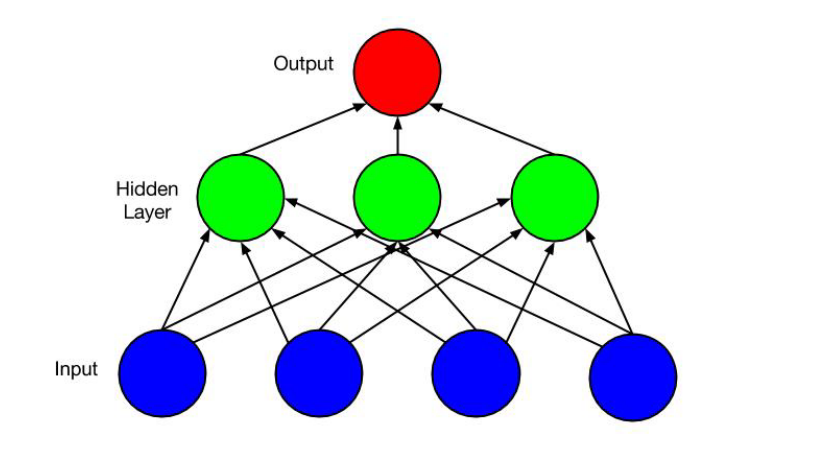
\includegraphics[width=0.7\textwidth]{./images/feedForwardNeuralNetwork.png}
  \end{center}
  \caption{Un modello di rete feedforward.
  Un campione \`e dato in pasto alla rete impostando i valori dei nodi blu.
  Ogni livello successivo \`e poi calcolato come una funzione dei livelli precedenti finch\`e non si raggiunge il livello pi\`u in alto.}
  \label{fig:feedforwardNeuralNetwork}
\end{figure}

L'input $x$ viene dato in pasto ad una rete neurale feedforward impostando i valori dei nodi del livello pi\`u in basso.
I valori dei nodi di ciascuno dei livelli superiori non potranno essere calcolati finch\`e non saranno disponibili i valori in output $\hat{y}$ dei livelli inferiori.
Queste tipologie di reti sono usate di frequente per applicazioni di apprendimento supervisionato come classificazione e regressione.
L'apprendimento \`e ottenuto aggiornando iterativamente i pesi dei singoli archi in modo da minimizzare una funzione di perdita, $\mathcal{L}(\hat{y},y)$, che penalizza la distanza fra l'output desiderato $y$ e l'output predetto $\hat{y}$ tramite tecniche di ottimizzazione.
Nonostante l'algoritmo di ottimizzazione esatto \`e un noto problema NP-Completo, una grande quantit\`a di euristiche pre addestramento e avanzate tecniche di ottimizzazione hanno condotto ad un impressionante numero di successi empirici su molte applicazioni di apprendimento supervisionato.

L'algoritmo utilizzato con maggiore successo per addestrare una rete neurale \`e l'algoritmo di back-propagation, introdotto da Rumelhart et al. nel 1985~\cite{Rumelhart:1985}.
Questo algoritmo usa la regola della \emph{catena} per calcolare la derivata di una funzione di perdita $\mathcal{L}$ rispetto ciascun parametro nella rete.
I pesi sui singoli archi vengono poi tramite la discesa dei gradienti.
Dato che la superficie di perdita non \`e convessa non vi \`e alcuna garanzia che l'algoritmo di back-propagation riesca a trovare un minimo globale.
Ci\`o nonostante, nella pratica, reti addestrate in questo modo hanno ottenuto notevoli successi.

Tuttavia le reti feedforward sono limitate.
Dopo che ciascun campione \`e stato processato l'intero stato della rete viene perso.
Se i campioni sono indipendenti gli uni dagli altri questo non presenta assolutamente un problema.
Ma se i dati sono in una relazione temporale, questo non \`e accettabile.
I fotogrammi di un video o le parole di una frase rappresentano situazioni in cui l'assunzione di indipendenza fallisce.

\section{Reti Neurali Ricorrenti}
Le \emph{reti neurali ricorrenti} costituiscono una estensione proprio delle reti neurali feedforward che, a differenza di quest'ultime, includono degli archi ricorrenti.
Questi archi ricorrenti si estendono su intervalli temporali adiacenti e introducono il concetto di tempo nel modello.
Mentre le RNN possono non contenere cicli tra gli archi convenzionali, gli archi ricorrenti possono formare cicli.
Al tempo $t$, i nodi che ricevono un input da un arco ricorrente, ricevono un \emph{input di attivazione} sia dal campione corrente $x^{(t)}$ che dai nodi nascosti $h^{(t-1)}$ del precedente stato della rete.
L'output $\hat{y}^{(t)}$ \`e poi calcolato in base allo stato nascosto $h^{(t)}$ del tempo $t$.
Quindi, l'input $x^{(t)}$ al tempo $t-1$ pu\`o influenzare l'output $\hat{y}^{(t)}$ al tempo $t$ proprio grazie a queste connessioni ricorrenti.

Le seguenti due equazioni, mostrano i calcoli necessari per eseguire, per ogni fase temporale, il passaggio in avanti dei dati di una semplice rete neurale ricorrente:
\begin{equation}
  h^{(t)} = \sigma(W_{hx}x + W_{hh}h^{(t-1)} + b_h)
\end{equation}
\begin{equation}
  \hat{y}^{(t)} = \operatorname{softmax}(W_{yh}h^{(t)} + b_y)
\end{equation}

dove $W_{hx}$ \`e la matrice dei pesi tra il livello di input e il livello nascosto mentre $W_{hh}$ \`e la matrice dei pesi ricorrenti fra i livelli nascosti di due fasi temporali adiacenti.
I vettori $b_h$ e $b_y$ rappresentano uno scostamento (\emph{bias}) che permettono a ciascun nodo di apprendere un offset.

I modelli discussi in questa tesi consistono in reti con livelli nascosti ricorrenti.
Tuttavia, sono stati proposti modelli, come la rete di Jordan, che ammettono la presenza di connessioni tra gli output della rete in uno stato e il livello nascosto della rete nello stato successivo.

\begin{figure}[tp]
  \centering
  \begin{center}
    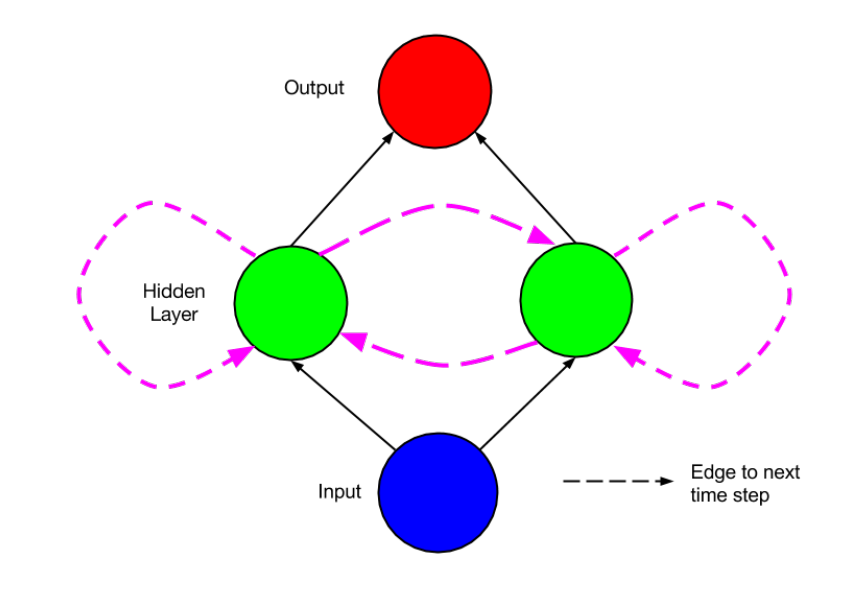
\includegraphics[width=0.7\textwidth]{./images/simpleRecurrentNeuralNetwork.png}
  \end{center}
  \caption{Una semplice rete neurale ricorrente.
  Ad ogni passo temporale $t$, l'attivazione viene passata lungo gli archi continui, cos\`i come accadrebbe per una normale rete feedforward.
  Gli archi tratteggiati collegano il nodo sorgente $j^{'}$ al tempo $t$, quindi $j^{'(t)}$, al nodo target del successivo passo temporale $j^{(t+1)}$.}
  \label{fig:simpleRecurrentNeuralNetwork}
\end{figure}

Una semplice rete neurale \`e mostrata in Figura~\ref{fig:simpleRecurrentNeuralNetwork}.
La dinamica di questa rete attraverso pi\`u fasi temporali pu\`o essere visualizzata \emph{dispiegando} la rete (Figura~\ref{fig:unfoldedSimpleRecurrentNeuralNetwork}).
Con questa visualizzazione, il modello pu\`o essere interpretata come una rete non ciclica, ma piuttosto come una rete con un livello per intervallo di tempo a dei pesi condivisi tra gli intervalli temporali.
Diventa quindi chiaro come una rete dispiegata in questo modo pu\`o essere addestrata attraverso pi\`u fasi temporali usando l'algoritmo di back-propagation.
Questo algoritmo viene chiamato \emph{back-propagation through time} (BPTT, back-propagation attraverso il tempo), ed \`e stata introdotta nel 1990~\cite{Werbos:1990}

\begin{figure}[tp]
  \centering
  \begin{center}
    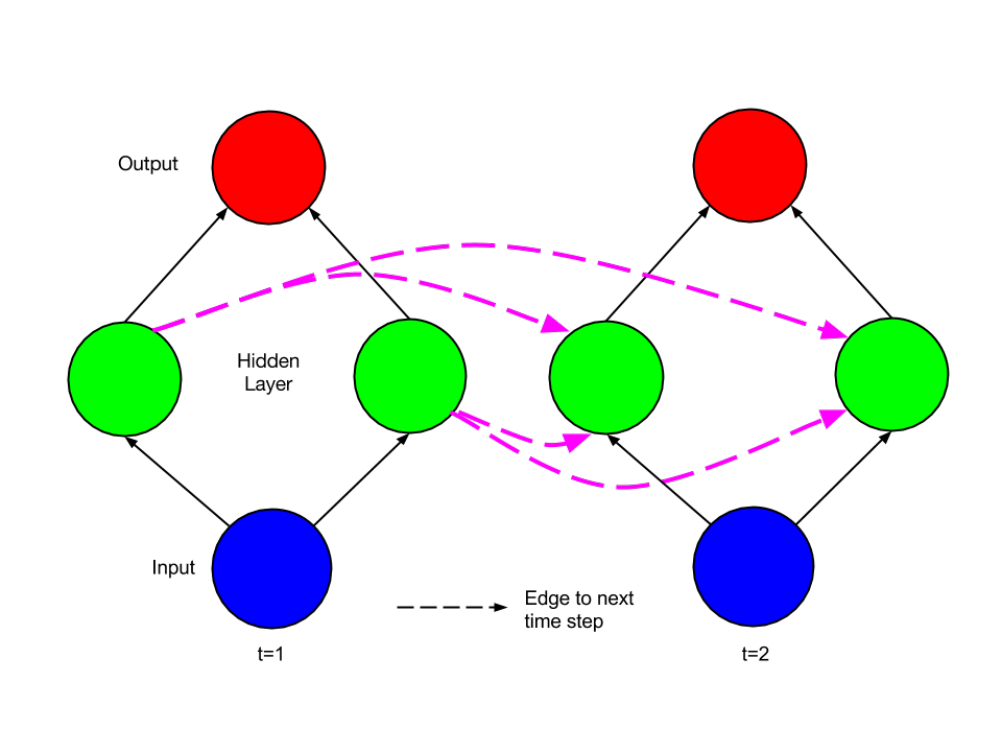
\includegraphics[width=0.7\textwidth]{./images/unfoldedSimpleRecurrentNeuralNetwork.png}
  \end{center}
  \caption{Visualizzazione della rete \emph{dispiegata}.}
  \label{fig:unfoldedSimpleRecurrentNeuralNetwork}
\end{figure}

% TODO QUI MANCA TUTTA LA PARTE DELLE JORDAN NETWORKS e tutta la letteratura sulle RNN
% http://arxiv.org/abs/1506.00019 ad esempio

\subsection{Addestramento}
L'apprendimento con le reti neurali ricorrenti \`e stato a lungo visto come qualcosa di difficile.
Cos\`i come per tutte le reti neurali, l'ottimizzazione della funzione di perdita \`e un problema NP-Completo.
Ma l'apprendimento con le reti ricorrenti pu\`o essere reso ancora pi\`u complesso a causa della difficolt\`a nell'apprendere delle dipendenze a lungo raggio.
Il noto problema della \emph{scomparsa} ed \emph{esplosione} dei gradienti si verifica quando l'errore viene propagato attraverso molte fasi temporali.
\mytodo{dire di pi\`u a riguardo?} L'impatto dell'input al tempo $\mathcal{T}$ sull'output al tempo $t$ esploder\`a esponenzialmente oppure raggiunger\`a rapidamente zero al crescere di $\mathcal{T} - t$, a seconda se il peso $\abs{w_{jj}}>1$ oppure $\abs{w_{jj}}<1$ ma anche in base alla funzione di attivazione utilizzata
(ad esempio con una funzione di attivazione $l_j = \sigma$ si verificher\`a maggiormente il problema della sparizione del gradiente, viceversa con la funzione ReLU $\operatorname{max}(0, x)$ il gradiente esploder\`a).

Una possibile soluzione al problema consiste nell'usare una versione leggermente modificate dell'algoritmo BPTT che prende il nome di \emph{truncated back-propagation through time} (TBPTT)~\cite{Williams:1989}.
Con l'algoritmo TBPTT viene impostato un valore che indicia il numero massimo di temporali lungo le quali pu\`o essere propagato l'errore.
In questo modo si attenua il problema dell'esplosione del gradiente perdendo, tuttavia, la capacit\`a di apprendere dipendenze a lungo raggio.

Il problema dell'ottimizzazione rappresenta un fondamentale ostacolo che non pu\`o essere risolto semplicemente modificando l'architettura della rete.
\`E noto dal 1993 che ottimizzare una rete neurale di anche solo 3 livelli costituisce un problema NP-Completo.
Tuttavia, recenti studi sia teorici che empirici, suggeriscono che il problema non \`e cos\`i insormontabile nella pratica come si potrebbe pensare.

Inoltre implementazioni sempre pi\`u performanti ed migliorate euristiche per il calcolo dei gradienti hanno reso l'addestramento delle RNN fattibile.
Ad esempio, implementazioni degli algoritmi di forward a backward propagation che sfruttano la GPU, come \emph{Theano} e \emph{Torch} (Sezione~\ref{sec:torch}), hanno semplificato la realizzazione di veloci algoritmi di apprendimento.
%Potresti parlare un po del modello di calcolo della GPU

\subsection{Architetture moderne}
Sono due le architetture RNN di maggior successo per l'apprendimento di dati sequenziali e risalgono entrambe al 1997.
La prima, \emph{Long Short-Term Memory}, ideata da Hochreiter e Schmidhuber, introduce il concetto di cella di memoria, un'unit\`a computazionale che rimpiazza il tradizionale neurone artificiale nei livelli nascosti della rete.
Con queste celle di memoria, la rete \`e in grado di superare le difficolt\`a incontrate dalle precedenti implementazioni durante la fase di apprendimento.
La seconda, \emph{Bidirectional Recurrent Neural Network}, ideata da Schuster e Paliwal, introduce invece l'architettura BRNN nella quale, per calcolare l'output del tempo $t$, vengono usate tanto le informazioni provenenti dal passato quanto quelle provenienti dal futuro.
Questo approccio \`e in contrasto con i sistemi precedenti, dove solo gli input provenienti da fasi temporali passate potevano influenzare gli output.
Fortunatamente, le due architetture non sono mutuamente esclusive e sono state combinate con successo.

Nel corso di questa tesi ci concentreremo sull'architettura \emph{Long Short-Term Memory}.

\section{Long Short-Term Memory (LSTM)}
Nel 1997, per superare il problema della scomparsa del gradiente, Hochreiter e Schmidhuber introdussero il modello LSTM.
Questo modello somiglia ad una rete neurale standard con un livello nascosto ricorrente, con l'unica differenza che i normali nodi di un livello nascosto (Figura~\ref{fig:artificialNeuron}) sono rimpiazzati da celle di memoria (Figura~\ref{fig:memoryCell}). %TODO immagini
La cella di memoria contiene un nodo sul quale insiste un un arco ricorrente connesso a se stesso con peso pari ad 1, assicurandosi, in questo modo, che il gradiente possa passare attraverso molte fasi temporali senza scomparire o esplodere.

\begin{figure}[tp]
  \centering
  \begin{center}
    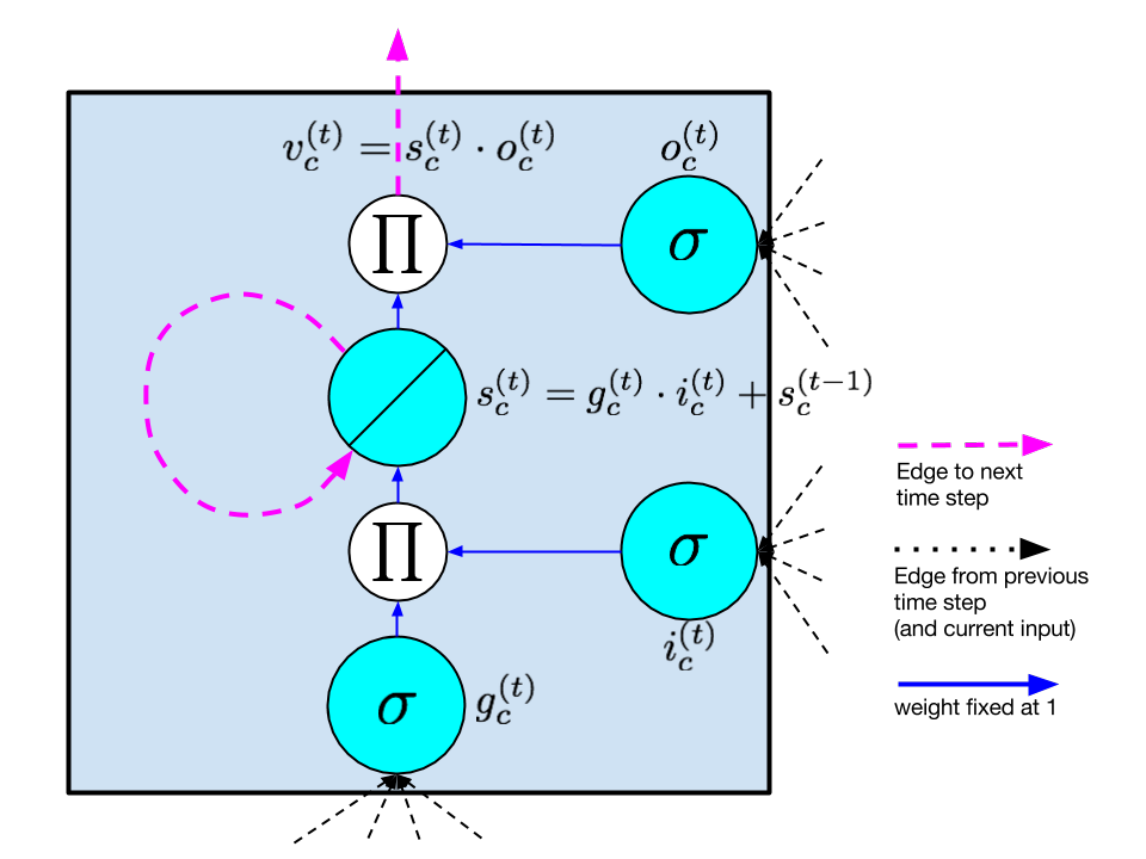
\includegraphics[width=0.7\textwidth]{./images/memoryCell.png}
  \end{center}
  \caption{Una cella di memoria del modello LSTM cos\`i come descritta inizialmente da Hochreiter et al. in~\cite{Hochreiter:1997}.
  Il nodo con l'arco ricorrente rappresenta lo stato interno $s$.
  La linea diagonale sta ad indicare che si tratta di una funzione lineare, non \`e applicata nessuna funzione di attivazione.
  I nodi con il simbolo ``$\prod$'' danno in output il prodotto degli input.
  Le linee tratteggiate indicano archi ricorrenti mentre quelle rosa hanno un peso costante pari ad 1.}
  \label{fig:memoryCell}
\end{figure}

Per distinguere la presenza di una cella di memoria da un nodo normale, indicheremo queste celle con $c$.

Il termine ``Long Short-Term Memory'' deriva dalla seguente intuizione.
Le reti neurali ricorrenti pi\`u semplici hanno una \emph{memoria a lungo termine} (\emph{long term memory}) sotto forma di pesi.
I pesi, durante l'apprendimento, cambiano molto lentamente, codificando, in questo modo, la conoscenza.
Queste hanno anche una \emph{memoria a breve termine} (\emph{short term memory}) sotto forma di attivazioni effimere, che passano dall'output di ciascun nodo nei nodi successivi.
Il modello LSTM introduce una sorta di memoria intermedia tramite l'uso delle celle di memoria.
Una cella di memoria \`e una composizione di unit\`a pi\`u semplici con la nuova aggiunta di nodi moltiplicativi, indicati nel diagramma con il simbolo $\prod$.
Di seguito sono descritti tutti gli elementi che compongono una cella di memoria.
\begin{itemize}
  \item \emph{Internal State:} Il cuore di ogni cella di memoria \`e un nodo $s$ con una funzione di attivazione lineare.
  Dato che indichiamo con $c$ una cella di memoria, il suo stato interno sar\`a indicato con $c_s$.
  \item \emph{Constant Error Carousel:} Lo stato interno $c_s$ ha un arco connesso a se stesso (ricorrente) con peso pari ad 1.
  Quest'arco, chiamato \emph{constant error carousel}, si estende tra fasi temporali adiacenti con un peso costante, questo assicura che l'errore possa passare attraverso le fasi temporali senza sparire o esplodere.
  \item \emph{Input Node:} Questo nodo si comporta come un normale nodo, prendendo gli input tanto dal resto della rete alla fase temporale precedente quanto dagli input al tempo corrente.
  Solitamente questo nodo viene indicato con $g$ e questa tesi non far\`a eccezione, anche se potrebbe generare confusione dato che sarebbe pi\`u appropriato usare $g$ per indicare i cancelli.
  \`E importante notare che quando usiamo la notazione vettoriale ci riferiamo ad un intero livello di celle.
  Ad esempio, $g$ \`e un vettore che contiene i valori di $g_c$ di tutte le celle in un dato livello.
  Quando, invece, usiamo il pedice $c$, allora ci riferiamo ad una singola cella di memoria.
  \item \emph{Multiplicative Gating:} I ``cancelli'' moltiplicativi (gates) sono una peculiarit\`a dei modelli LSTM.
  Qu\`i un'unit\`a sigmoidale chiamata \emph{gate} viene addestrata dato l'input e una connessione ricorrente in arrivo dal passo temporale precedente.
  Alcuni valori di interesse sono poi moltiplicati per l'output di questa unit\`a.
  Se il cancello da in output 0, allora questo \`e chiuso e il flusso dei dati viene interrotto.
  Se, invece, da in output 1 allora in cancello \`e aperto e il flusso dei dati pu\`o passarci attraverso.
  Il modello LSTM originale prevedeva due cancelli:
  \begin{itemize}
    \item \emph{Input Gate:} Il primo \`e l'\emph{input gate} $i_c$, che \`e moltiplicato per il nodo input $g_c$
    \item \emph{Output Gate:} Il secondo cancello \`e chiamato \emph{output gate} $o_c$.
    Questo viene moltiplicato per il valore dello stato interno $s_c$ per produrre il valore in output $v_c$ della cella di memoria.
    Questo poi viene dato in pasto al livello nascosto della LSTM nel prossimo passo temporale $h^{(t+1)}$ insieme all'output $\hat{y}^(t)$ generato al passo corrente.
  \end{itemize}
  Questi cancelli vengono indicati con $y_{in}$ e $y_{out}$, tuttavia questa notazione genera confusione perch\`e $y$ \`e solitamente utilizzato per indicare l'output nella letteratura di machine learning.
  Per questo motivo utilizzeremo le notazioni $i$, $o$ ed $f$ per indicare i cancelli di \emph{input}, \emph{output} e \emph{forget} (di cui pareler\`o a breve).
\end{itemize}

\begin{figure}[tp]
  \centering
  \begin{center}
    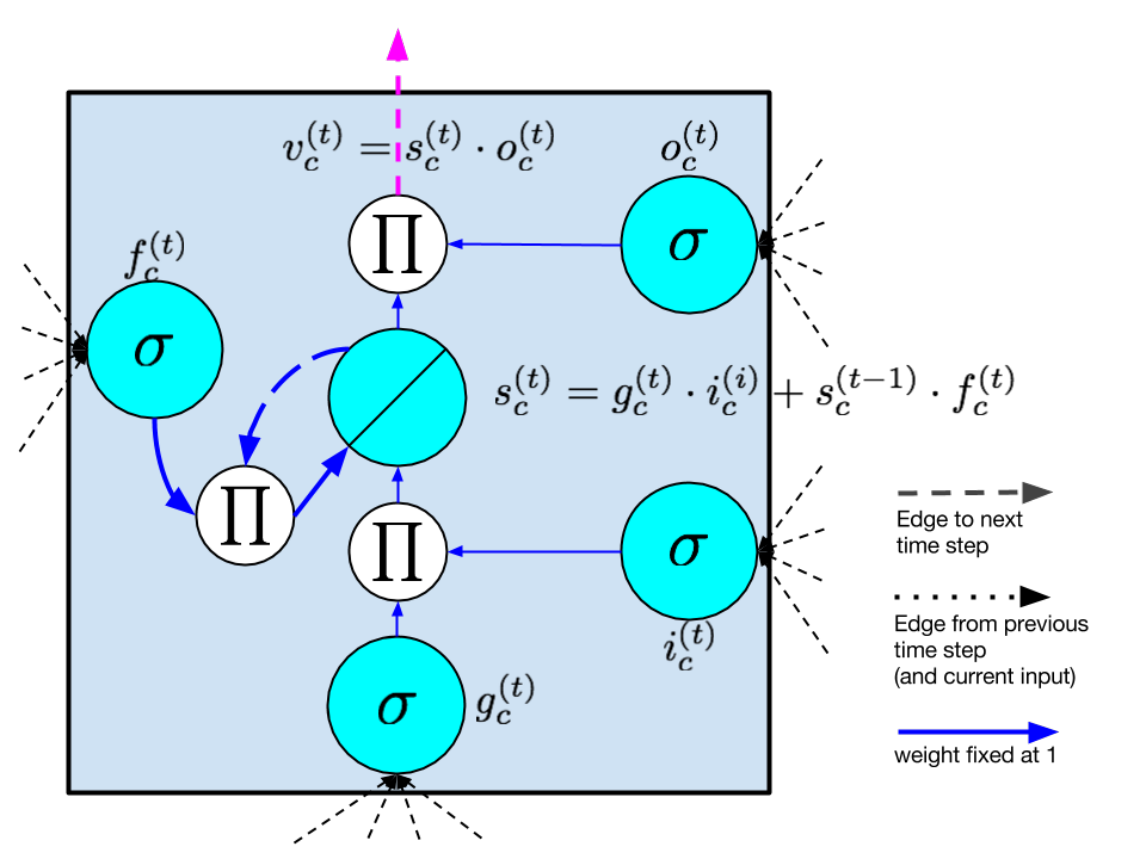
\includegraphics[width=0.7\textwidth]{./images/memoryCellWithForgetGate.png}
  \end{center}
  \caption{Una cella di memoria del modello LSTM con il \emph{forget gate} cos\`i come descritta da Gers et al. in~\cite{Gers:2000}.}
  \label{fig:memoryCellWithForgetGate}
\end{figure}

Fin da quando \`e stato proposto il modello LSTM originale, molte varianti sono state proposte.
Il \emph{forget gate}, proposti nel 2000 da Gers e Schmidhuber~\cite{Gers:2000}, aggiunge un cancello simile a quelli di input e output che permette, alla rete neurale, di svuotare le informazioni presenti nel \emph{constant error carousel}.
In altre parole, questo ulteriore cancello da alla LSTM la capacit\`a di apprendere quando ``dimenticare'' le informazioni ottenute dalle precedenti fasi temporali.
Il \emph{forget gate} \`e diventato di uso comune, un pilastro dei successivi lavori sulle LSTM.

Formalmente, la computazione in una LSTM procede in accordo ai seguenti calcoli che devono essere valutati ad ogni fase temporale.
Queste equazioni forniscono l'algoritmo completo per una moderna LSTM, comprensiva di forget gate.
\begin{equation}
  g^{(t)} = \phi(W_{gx}x^{(t)} + W_{ih}h^{(t-1)} + b_g)
\end{equation}
\begin{equation}
  i^{(t)} = \sigma(W_{ix}x^{(t)} + W_{ih}h^{(t-1)} + b_i)
\end{equation}
\begin{equation}
  f^{(t)} = \sigma(W_{fx}x^{(t)} + W_{fh}h^{(t-1)} + b_f)
\end{equation}
\begin{equation}
  o^{(t)} = \sigma(W_{ox}x^{(t)} + W_{oh}h^{(t-1)} + b_o)
\end{equation}
\begin{equation}
  s^{(t)} = g^{(t)} \odot i^{(t)} + s^{(t-1)} \odot f^{(t)}
\end{equation}
\begin{equation}
  h^{(t)} = s^{(t)} \odot o^{(t)}
\end{equation}

dove $\odot$ sta per moltiplicazione elemento per elemento.
Il calcolo di una LSTM semplice, senza forget gate, \`e dato impostando $f^{(t)} = 1$ per ogni $t$.
Seguendo l'ultimo stato dell'arte abbiamo usato la funzione tanh $\phi$ per i nodi di input $g$, nonostante l'implementazione originale del modello LSTM prevedesse l'uso di una funzione sigmoide $\sigma$~\cite{Hochreiter:1997}.
Ancora, $h^{(t-1)}$ \`e un vettore contenente i valori $v_c$ dati in output da ciascuna cella di memoria $c$ del livello nascosto dalla precedente fase temporale.

Intuitivamente, in termini di forward pass dei dati, il modello LSTM pu\`o apprendere quando lasciar passare l'attivazione nello stato interno.
Fintantoch\`e il cancello di input (\emph{input gate}) resta chiuso (da in output 0), nessuna attivazione pu\`o passare.
Allo stesso modo, il cancello di output (\emph{output gate}) apprende quando lasciar uscire il valore dello stato interno.
Quando entrambi i cancelli sono \emph{chiusi}, l'attivazione rimane confinata, senza subire modifiche ne, tantomeno, influenzare l'output delle fasi temporali intermedie.
In termini di \emph{backward pass}, il \emph{constant error carousel} permette al gradiente di poter essere propagato attraverso molte fasi temporali, senza sparire o esplodere.
In quest'ottica, quindi, i cancelli apprendono quando lasciar entrare l'\emph{errore} e quando lasciarlo uscire.
Nella pratica, il modello LSTM ha dimostrato un'abilit\`a superiore nell'apprendere dinepndenze a lungo raggio, rispetto alle normali RNN.
Di conseguenza, questo modello, \`e diventato l'attuale stato dell'arte nel campo delle reti neurali.

\section{Torch7}
\label{sec:torch}
\nocite{Collobert:2011}

Torch7 \`e un framework di cumputazione numerica e una libreria di machine learning che estende \emph{Lua}, progettato per rispondere, principalmente, a tre esigenze:
\begin{enumerate}
  \item deve permettere un \emph{facile sviluppo di algoritmi numerici}
  \item deve essere \emph{facile da estendere} (incluso l'uso di altre librerie)
  \item deve essere \emph{veloce}
\end{enumerate}

\subsection{Perch\`e Lua?}
L'uso di un linguaggio di scripting (interpretato) con \emph{buone API C} sembra essere la scelta migliore per soddisfare il requisito (2).
Innanzitutto, un linguaggio ad alto livello rende lo sviluppo di programmi pi\`u semplice e pi\`u comprensibile rispetto ad uno a basso livello.
In secondo luigo, se il linguaggio di programmazione \`e \emph{interpretato}, diventa pi\`u facile provare velocemente varie idee in maniera interattiva.
In fine, con la presenza di buone API C, il linguaggio di scripting diventa il ``collante'' fra varie librerie in diversi linguaggi: differenti modellazioni dello stesso concetto (provenienti da diverse librerie) possono essere nascoste dietro un unico modello realizzato con il linguaggi di scripting, pur mantenendo tutte le funzionalit\`a di tutte le librerie.

Fra tutti i linguaggi di scripting l'unico che pu\`o soddisfare il vincolo (3) \`e Lua.
Lua \`e, infatti, il linguaggio interpretato pi\`u veloce (con anche il pi\`u veloce compilatore Just In Time (JIT)).
Lua ha anche il vantaggio di essere stato progettato per essere facilmente \emph{incorporato} in applicazioni scritti in C, e fornisce dele ottime API C.

\textbf{Lua} \`e stato pensato per essere usato come un potente e leggero linguaggio di scripting per ogni programma che ne avesse bisogno, ed \`e stato implementato a mo' di una libreria scritta in C.
Citando la pagina web di lua:

\begin{quote}
Lua combines simple procedural syntax with powerful data description constructs based on associative arrays and extensible semantics. Lua is dynamically typed, runs by interpreting bytecode for a register-based virtual machine, and has auto- matic memory management with incremental garbage collection, making it ideal for configuration, scripting, and rapid prototyping.
\end{quote}

Lua offre un discreto supporto alla programmazione object-oriented, alla programmazione funzionale e alla programmazione data-driven.
Il tipo principale di Lua \`e la tabella, che implementa un array associativo in maniera molto efficiente.
Un array associativo altro non \`e che un array i cui indici possono essere non solo numeri, ma anche stringhe o qualsiasi altro dipo di valore che il linguaggio mette a disposizione.
Queste tabelle non hanno una dimensione fissa, possono essere ridimensionate in maniera dinamica, e possono essere usate come ``tabelle virtuali'' per altre tabelle, permettendo, in questo modo, di simulare alcune delle caratteristiche del paradigma object-oriented (come ad esempio l'ereditariet\`a).
Inoltre \`e l'unica struttura dati presente in Lua, ma \`e molto potente e flessibile, viene utilizzata per rappresentare semplici array, insiemi, record, code e molte altre strutture dati, in maniera semplice, unoforme ed efficiente.

\subsection{La Classe Tensor}
Torch7 si basa fortemente sulla sua classe \emph{Tensor} (Tensore), che estende l'insieme dei tipi di base di Lua, fornendo un'efficiente implementazione di un array multi dimensionale.
Gran parte delle librerie scritte per Torch7 usano la sua classe Tensor per rappresentare dati come segnali, immagini, video ecc. .
La libreria Tensor di Torch7 fornisce numerose operazioni (fra cui molte operazioni di algebra lineare), implementate efficientemente in C, che sfruttano l'insieme di istruzioni SSE su piattaforma Intel e, optionalmente, sfruttando le performanti implementazioni BLAS/Lapack (come Intel MKL) per eseguire operazioni di algebra lineare.

Di seguito alcune operazioni standard eseguibili con la classe Tensor:

\lstinputlisting[language={[5.0]Lua}]{snippets/tensor.lua}

Inoltre, cos\`i come in matlab, pi\`u tipi possono coesistere in Torch7 ed \`e semplice passare da un tipo ad un altro:

\lstinputlisting[language={[5.0]Lua}]{snippets/tensor_conversions.lua}

\subsection{Pacchetti utilizzati}

Di seguito la lista delle librerie utilizzate nel coros di questa tesi:

\subsubsection{luautf8}
La libreria \emph{luautf8} espone numerose funzione per manipolare stringhe con codifica utf8.

\subsubsection{torch}
La libreria principale di Torch7: fornisce la class Tensor, strumenti per la serializzazione e altre funzionalit\`a di base.

\subsubsection{nn}
La libreria \emph{nn} fornisce un insieme di moduli standard per il calcolo di reti neurali, oltre ad un insieme di moduli contenitori che possono essere usati per definire qualsivoglia grafo diretto (aciclico o no).
Tramite una descrizione diretta dell'architettura dei grafi, usando dei moduli che sono componibili, si evita la complessit\`a di utilizzare un parser per interpretare il grafo o di creare un compilatore middle-ware.
In pratica, la maggior parte delle reti sono o sequenziali, o hanno una struttura ad albero semplice con ricorsioni.
Il seguente esempio descrive un percettrone multi livello:

\lstinputlisting[language={[5.0]Lua}]{snippets/multilayer_perceptron.lua}

Dove \lstinline[language={[5.0]Lua}]|nn.Sequential()| \`e un contenitore che definisce una rete neurale sequenziale, mentre \lstinline[language={[5.0]Lua}]|nn.Linera()|, \lstinline[language={[5.0]Lua}]|nn.Tanh()| e \lstinline[language={[5.0]Lua}]|nn.SoftMax()| sono i moduli che definiscono i singoli livelli del percettrone.
Ogni modulo, o contenitore, mette a disposizione delle funzioni standard per calcolare il suo output, e funzioni per calcolare le derivate da propagare indietro verso propri input e i prori parametri interni durante la backward pass.
Data la rete definita in precedenza, un input $X$, il gradiente $\partial E / \partial \hat{Y}$ calcolato da un errore $E$ e da un output generato $\hat{Y}$, queste tre funzioni possono essere eseguiti nel seguente modo:

\lstinputlisting[language={[5.0]Lua}]{snippets/forward_backward_pass.lua}

Dove \lstinline[language={[5.0]Lua}]|loss| \`e una qualche funzione di perdita.

\subsubsection{nngraph}
Un estensione della libreria \emph{nn} che semplifica la creazione di architetture neurali complesse.

\subsubsection{optim}
Una librerie che fornisce implementazioni per la discesa del gradiente, per il metodo del gradiente coniugato e altri algoritmi di ottimizzazione.

\subsection{Efficienza}

Torch7 \`e stato progettato pensando principalmente all'efficienza, infatti sfrutta, quando \`e possibile, l'insieme di istruzione \emph{SSE} e supporta due meccanismi di parallelizzazione: \emph{OpenMP} e \emph{CUDA}.
La libreria Tensor fa un uso massiccio di queste tecniche.
Dal punto di vista dell'utente, abilitare CUDA e OpenMP pu\`o portare ad un massiccio incremento delle prestazioni con qualsiasi script ``Lua'', senza alcuno sforzo aggiuntivo, proprio perch\`e la maggior parte delle librerie dipendono dalla libreria Tensor.
Altre libreria (come la libreria \emph{nn}) fanno comunque uso di OpenMP e CUDA anche quando non fanno uso della libreria Tensor.

\subsubsection{CUDA}
Per gli esperimenti svolti durante questa tesi \`e stata utilizzata la tecnologia CUDA.
CUDA (Compute Unified Device Architecture) \`e un framework proprietario nVidia, utilizzato per programmare i loro processori grafici e sfruttarli per eseguire calcoli general purpose, non legati strettamente alla grafica.
CUDA permette di controllare l'intera gerarchia di memoria disponibile al processore grafico, di cui, i due maggiori componento sono la DRAM, una grande memoria esterna ad alta latenza, e la memoria interna al processore, a bassa latenza ma dell'ordine di qualche KB.
Inoltre permette di controllare anche l'intera gerarchida dei core del processore, nonch\`e i meccanismi di interazione con ciascun core, e con le differenti tipologie di memoria.

Per sfruttare CUDA, Torch7 mette a disposizione un nuovo tipo di tensore: \lstinline[language={[5.0]Lua}]|torch.CudaTensor|.
Una volta creato, questo tensore viene memorizzato nella memora DRAM della GPU.
Tutte le operazioni valide per un normale Tensor lo sono anche per un CudaTensor, che astrae completamente l'uso del processore grafico.
